\section{Combination of Mixed Precision and Low-Rank}
\label{sec:combination}

After establishing low-rank approximations as a viable alternative to factorization in lower precision, the natural question arises of whether or not it is viable to combine both approaches. This section is dedicated to the investigation of such a environment, aiming to examine the viability of low-rank low precision methods. It is also the reason why half precision arithmetics were not considered in the experimental settings, since those are not supported by the library used for hierarchical approximations in this research. The basic workflow is similar to iterative refinement in three precisions:
\begin{itemize}
    \item $u_f$ : single precision for the calculation of the hierarchical LU factorization
     \item $u$ : double precision for most of the other steps (the result should also accurate to this precision)
     \item $u_r$ : quadruple precision for calculating the residuals and some calculations within GMRES
\end{itemize}

\noindent The same set of test matrices as in Section~\hyperref[sec:low_rank_ir]{\ref{sec:low_rank_ir}} was used, converting them to single precision before the factorization. It is noteworthy, that in order to provide a fair comparison, the rank of the low-rank approximations was not adjusted. This can result in a (slightly) larger $\epsilon$ for the single precision hierarchical representation. However, changing the rank would also change the associated workload, making the two variants more difficult to compare. Furthermore, as indicated by the results of the previous section, similar behaviour can be expected for equal values of $\epsilon$ as long as $\epsilon > u_f$. This hypothesis is supported by the actual results depicted in Figures~\hyperref[fig:lrirs1]{\ref{fig:lrirs1}} - \hyperref[fig:lrirs4]{\ref{fig:lrirs4}}. The plots show a comparison of the errors obtained by LU-based iterative refinement with the factorization being calculated in either double or single precision for matrices of dimension $512 \times 512$ and varying condition number.

\begin{figure}
\centering
\begin{subfigure}{.5\textwidth}
  \centering
  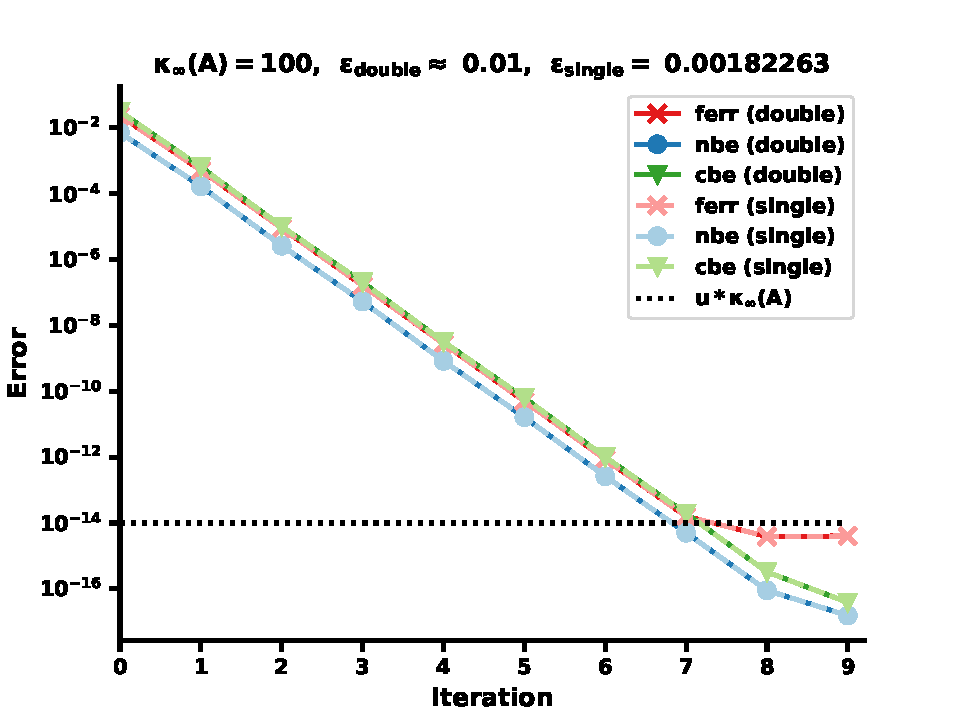
\includegraphics[width=\linewidth]{chapters/5_experiments/figures/LU512_e0_0s.pdf}
  \caption{$\epsilon_{double} \approx 10^{-2}$}
  \label{fig:lrirs1_1}
\end{subfigure}%
\begin{subfigure}{.5\textwidth}
  \centering
  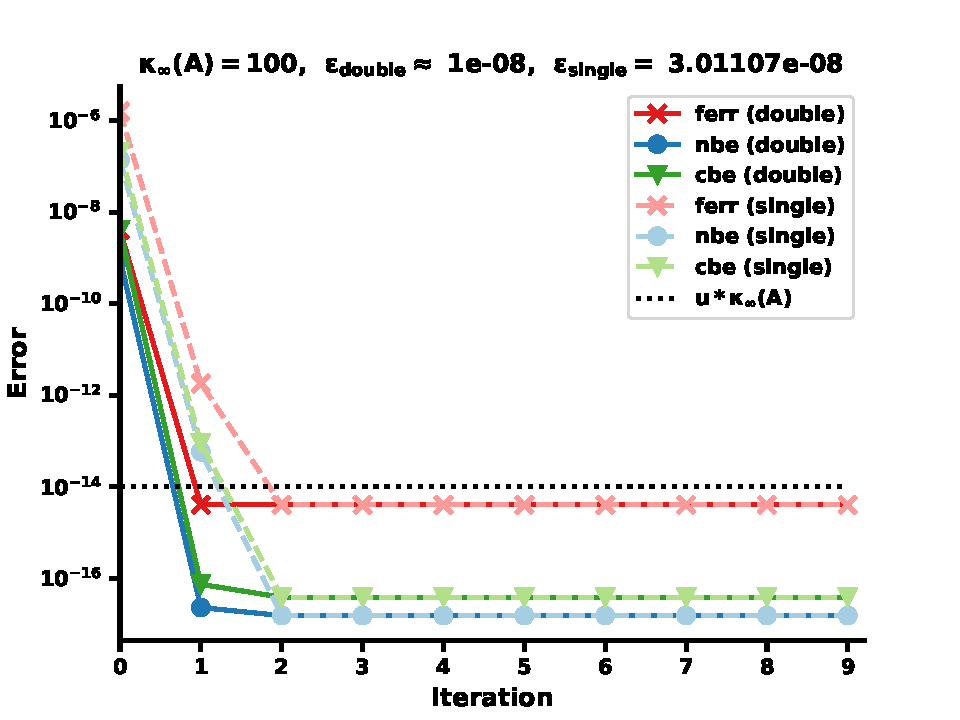
\includegraphics[width=\linewidth]{chapters/5_experiments/figures/LU512_e0_1s.pdf}
  \caption{$\epsilon_{double} \approx 10^{-8}$}
  \label{fig:lrirs1_2}
\end{subfigure}
\caption[Mixed Precision Low-Rank LU-IR 1]{Comparison of hierarchical LU factorization in single and double precision. Measurements are obtained from a LU-based IR where $\kappa_\infty(A) \approx 10^2$.}
\label{fig:lrirs1}
\end{figure}

\begin{figure}
\centering
\begin{subfigure}{.5\textwidth}
  \centering
  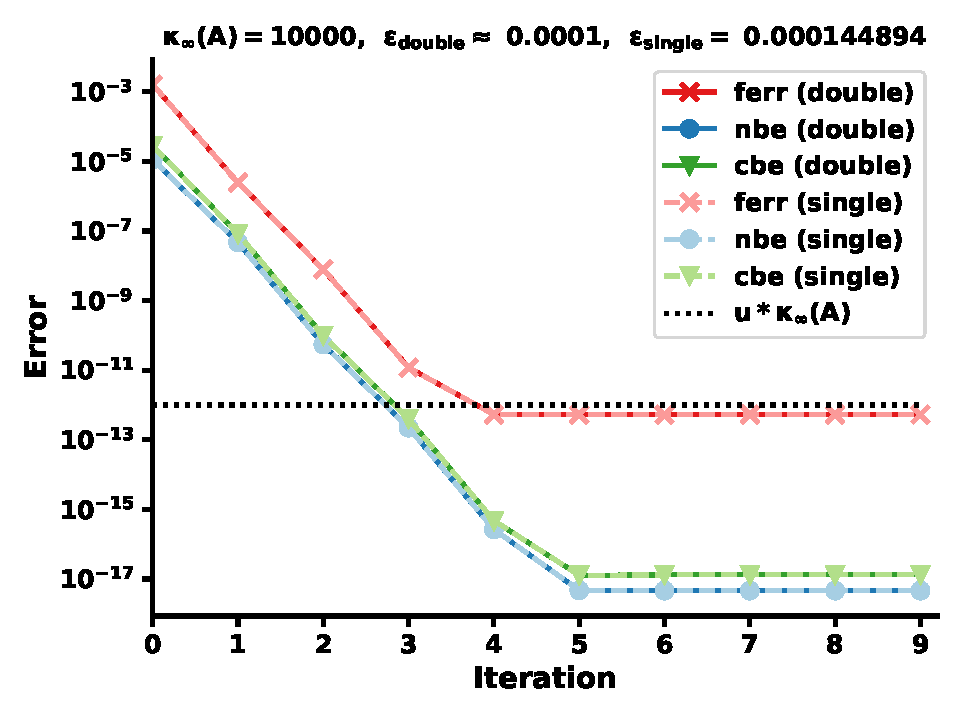
\includegraphics[width=\linewidth]{chapters/5_experiments/figures/LU512_e1_0s.pdf}
  \caption{$\epsilon_{double} \approx 10^{-4}$}
  \label{fig:lrirs2_1}
\end{subfigure}%
\begin{subfigure}{.5\textwidth}
  \centering
  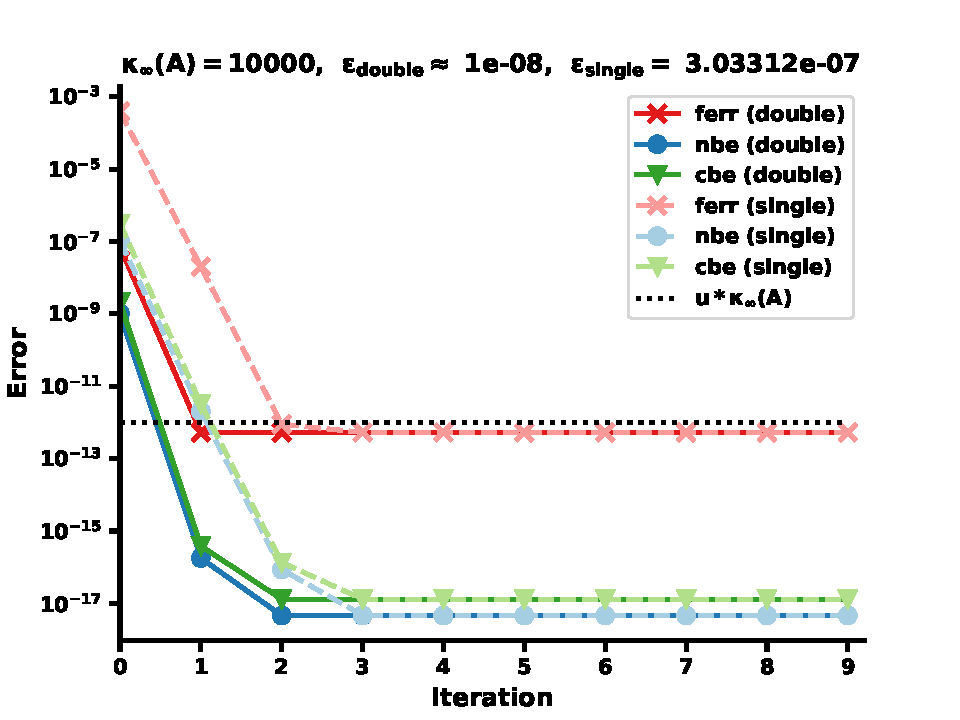
\includegraphics[width=\linewidth]{chapters/5_experiments/figures/LU512_e1_1s.pdf}
  \caption{$\epsilon_{double} \approx 10^{-8}$}
  \label{fig:lrirs2_2}
\end{subfigure}
\caption[Mixed Precision Low-Rank LU-IR 2]{Comparison of hierarchical LU factorization in single and double precision. Measurements are obtained from a LU-based IR where $\kappa_\infty(A) \approx 10^4$.}
\label{fig:lrirs2}
\end{figure}

Figures~\hyperref[fig:lrirs1_1]{\ref{fig:lrirs1_1}} \& \hyperref[fig:lrirs1_2]{\ref{fig:lrirs1_2}} illustrate the general case for $\kappa_\infty(A)<u_f^{-1}$. As long as the condition number of $A$ is lower than the reciprocal of the factorization precision, LU-based iterative refinement converges, even for very small values of $\epsilon$. The number of necessary iterations, on the other side is directly dependent on the approximation accuracy $\epsilon$ with a higher accuracy requiring less steps. The implications of lower precision factorization can be clearly observed in Figure~\hyperref[fig:lrirs3_2]{\ref{fig:lrirs3_2}}. The lower precision (for the same rank) induces a higher value of $\epsilon$, which increases the number of iterations before convergence by one. This issue would most likely disappear, if the rank was increased until an equally accurate hierarchical representation was achieved. Note, however, that $\epsilon$ is limited by $u_f$ and con not be increased arbitrarily.

\begin{figure}
\centering
\begin{subfigure}{.5\textwidth}
  \centering
  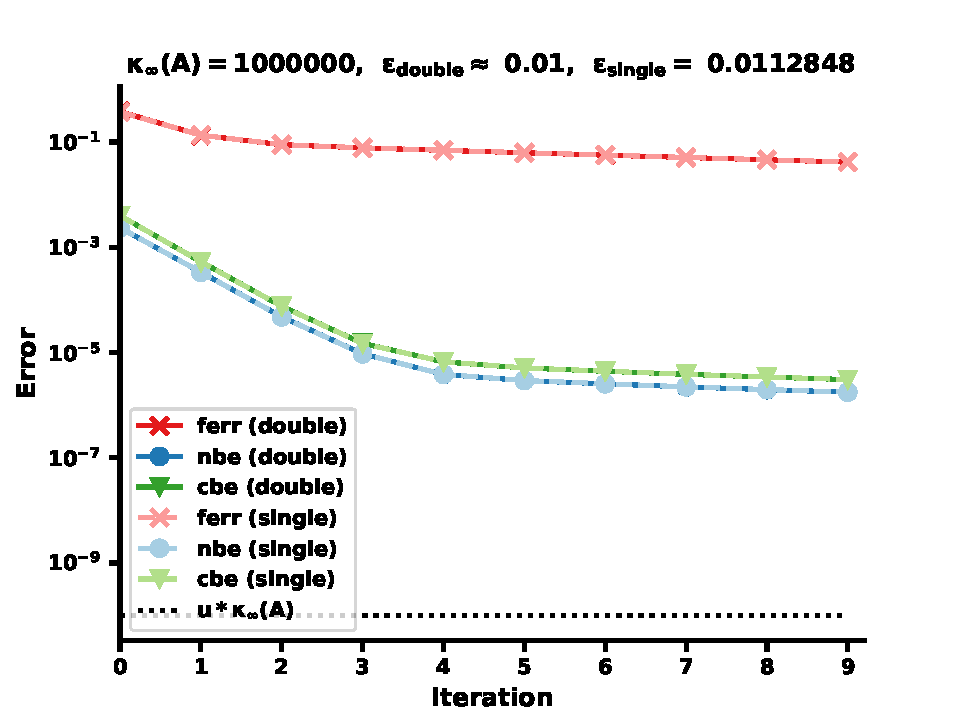
\includegraphics[width=\linewidth]{chapters/5_experiments/figures/LU512_e2_0s.pdf}
  \caption{$\epsilon_{double} \approx 10^{-2}$}
  \label{fig:lrirs3_1}
\end{subfigure}%
\begin{subfigure}{.5\textwidth}
  \centering
  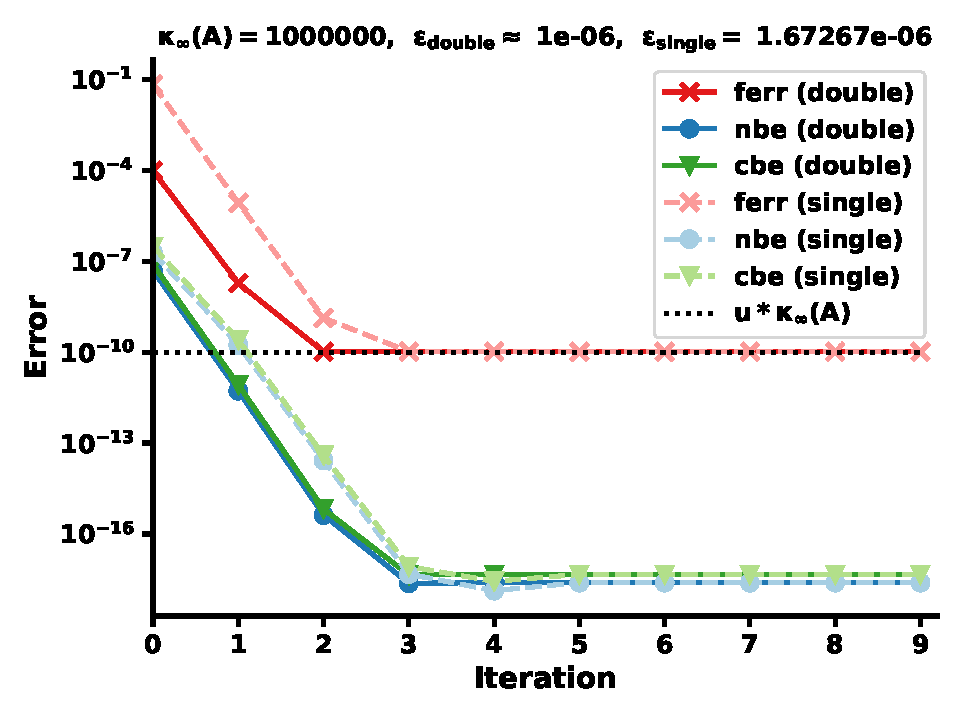
\includegraphics[width=\linewidth]{chapters/5_experiments/figures/LU512_e2_1s.pdf}
  \caption{$\epsilon_{double} \approx 10^{-6}$}
  \label{fig:lrirs3_2}
\end{subfigure}
\caption[Mixed Precision Low-Rank LU-IR 3]{Comparison of hierarchical LU factorization in single and double precision. Measurements are obtained from a LU-based IR where $\kappa_\infty(A) \approx 10^6$.}
\label{fig:lrirs3}
\end{figure}

\begin{figure}
\centering
\begin{subfigure}{.5\textwidth}
  \centering
  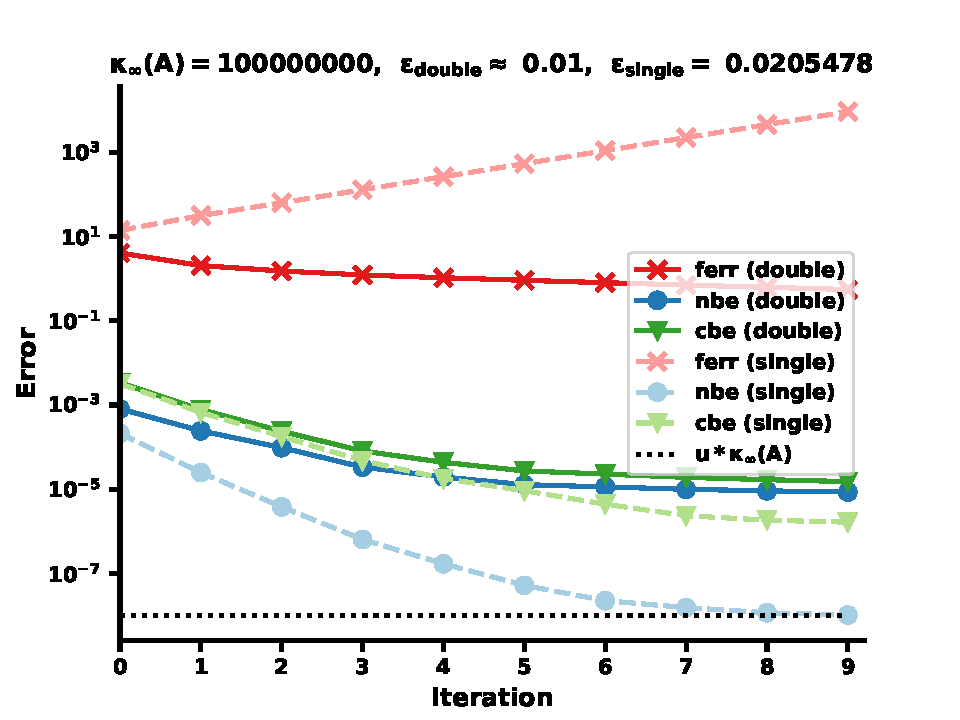
\includegraphics[width=\linewidth]{chapters/5_experiments/figures/LU512_e3_0s.pdf}
  \caption{$\epsilon_{double} \approx 10^{-2}$}
  \label{fig:lrirs4_1}
\end{subfigure}%
\begin{subfigure}{.5\textwidth}
  \centering
  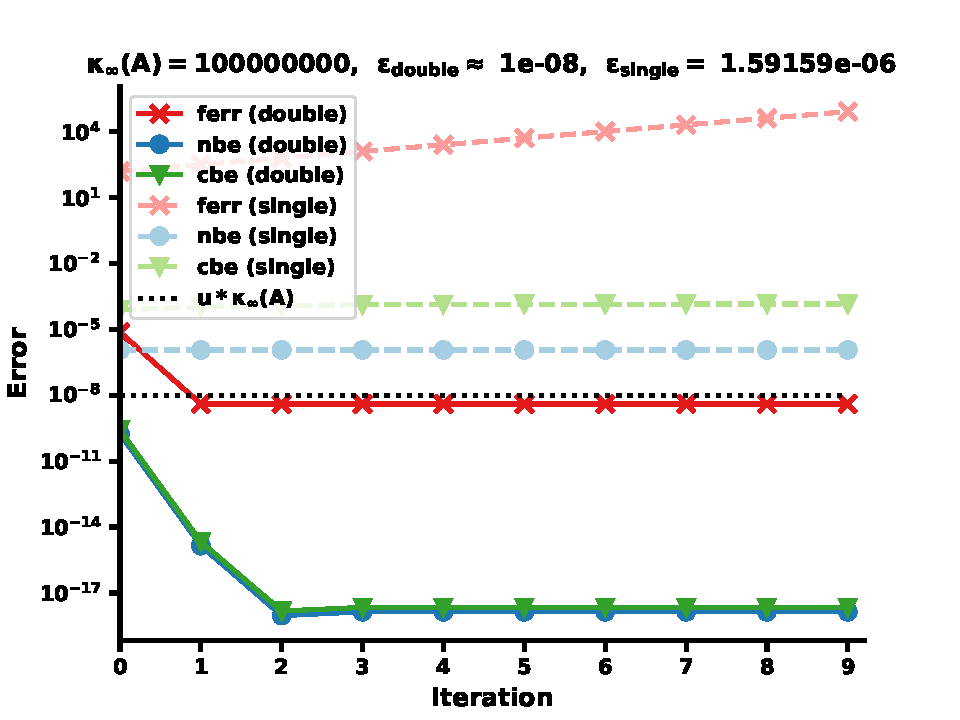
\includegraphics[width=\linewidth]{chapters/5_experiments/figures/LU512_e3_1s.pdf}
  \caption{$\epsilon_{double} \approx 10^{-8}$}
  \label{fig:lrirs4_2}
\end{subfigure}
\caption[Mixed Precision Low-Rank LU-IR 4]{Comparison of hierarchical LU factorization in single and double precision. Measurements are obtained from a LU-based IR where $\kappa_\infty(A) \approx 10^8$.}
\label{fig:lrirs4}
\end{figure}

The same disadvantages as with ordinary LU-based iterative refinement (see Section~\hyperref[sec:mixed_precision]{\ref{sec:mixed_precision}}) become visible if $A$ is very ill-conditioned. With $\kappa_\infty(A) \geq u_f^{-1}$, the mixed precision variant breaks down and starts to diverge, while IR refinement based on a double precision low-rank approximation still converges. This behaviour can be seen in Figures~\hyperref[fig:lrirs4_1]{\ref{fig:lrirs4_1}} \& \hyperref[fig:lrirs4_2]{\ref{fig:lrirs4_2}}. Even though this is the general case, it needs to be mentioned that for a single test-case, convergence was observed despite the high condition number, but the contributing factors remain (as of yet) unclear and further investigation is necessary. Overall, LU-based IR with a hierarchical factorization is able to deliver similar results to standard IR in three precisions and it seems like the same error bounds are applicable. 

The same assertion can be made for GMRES-based IR refinement, where similar results are obtained for the hierarchical and general case. In contrast to LU-based IR, this variant does not break down even if $\kappa_\infty(A) \geq u_f^{-1}$ and convergence for single precision factorization does not seem to differ much from the double precision case. This is clearly demonstrated in Figures~\hyperref[fig:lrirsg3_1]{\ref{fig:lrirsg3_1}} \& \hyperref[fig:lrirsg3_2]{\ref{fig:lrirsg3_2}}, where the single precision factorization achieves the same error bounds as the more accurate double one. For the less crucial condition numbers, the general trend of GMRES-based IR is displayed in Figures~\hyperref[fig:lrirsg1]{\ref{fig:lrirsg1}} - \hyperref[fig:lrirsg3]{\ref{fig:lrirsg3}}, showing that there is basically no difference in the errors for both variants.

\begin{figure}
\centering
\begin{subfigure}{.5\textwidth}
  \centering
  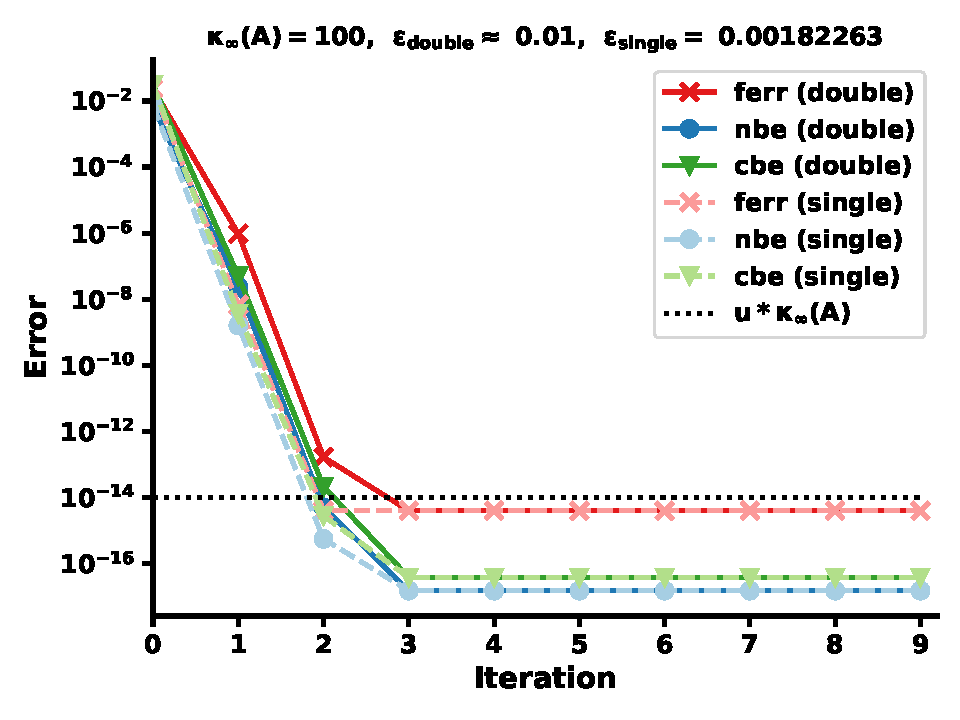
\includegraphics[width=\linewidth]{chapters/5_experiments/figures/GMRES512_e0_0s.pdf}
  \caption{$\epsilon_{double} \approx 10^{-2}$}
  \label{fig:lrirsg1_1}
\end{subfigure}%
\begin{subfigure}{.5\textwidth}
  \centering
  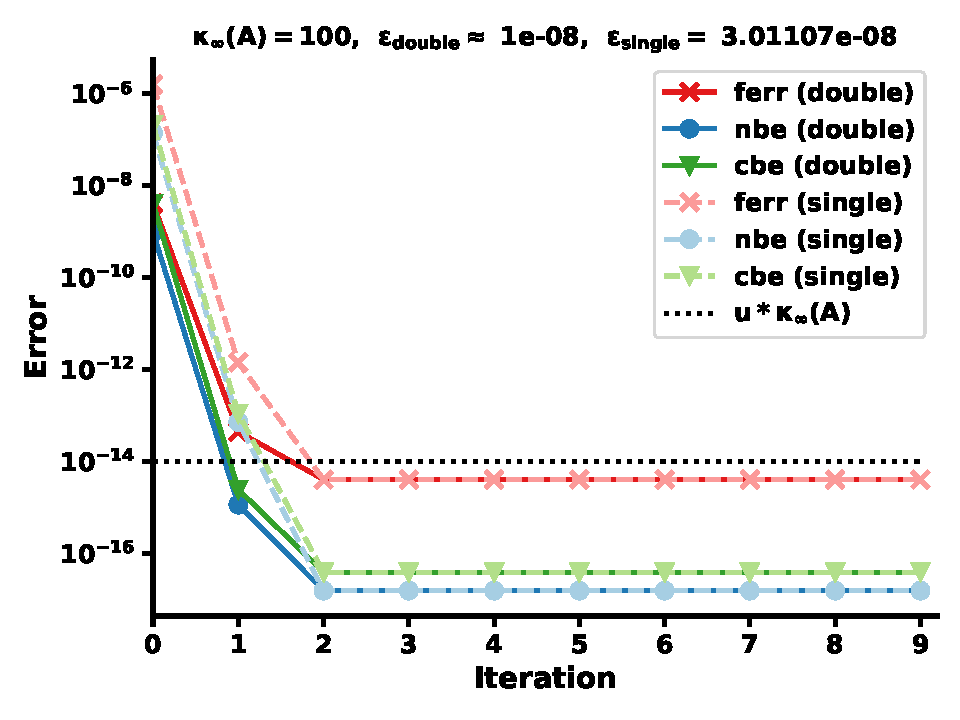
\includegraphics[width=\linewidth]{chapters/5_experiments/figures/GMRES512_e0_1s.pdf}
  \caption{$\epsilon_{double} \approx 10^{-8}$}
  \label{fig:lrirsg1_2}
\end{subfigure}
\caption[Mixed Precision Low-Rank GMRES-IR 1]{Comparison of hierarchical LU factorization in single and double precision. Measurements are obtained from a GMRES-based IR where $\kappa_\infty(A) \approx 10^2$.}
\label{fig:lrirsg1}
\end{figure}

\begin{figure}
\centering
\begin{subfigure}{.5\textwidth}
  \centering
  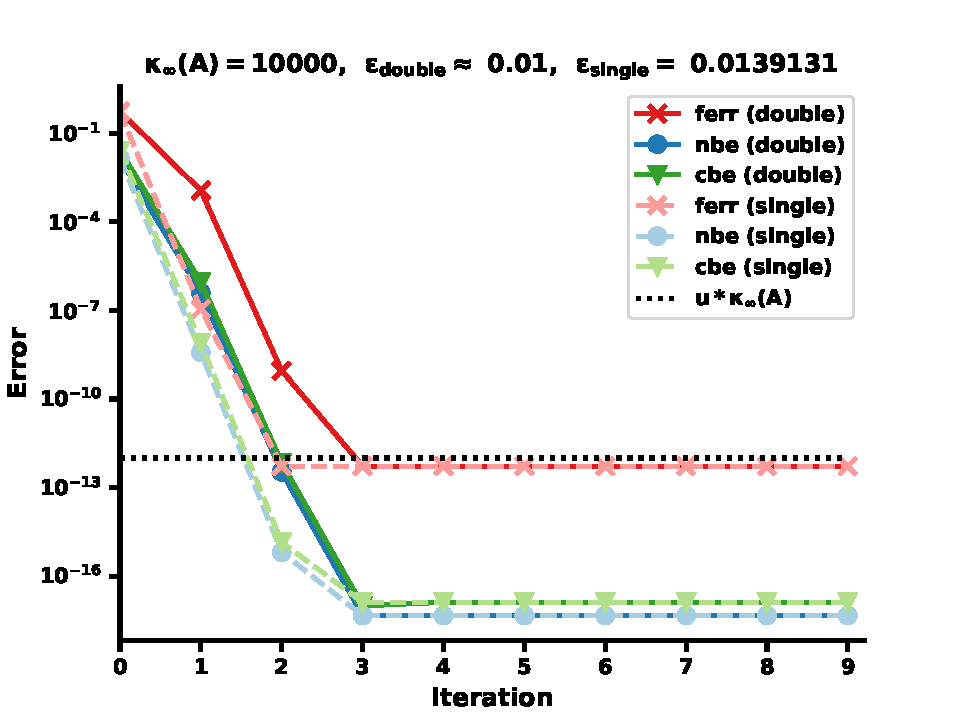
\includegraphics[width=\linewidth]{chapters/5_experiments/figures/GMRES512_e1_0s.pdf}
  \caption{$\epsilon_{double} \approx 10^{-2}$}
  \label{fig:lrirsg2_1}
\end{subfigure}%
\begin{subfigure}{.5\textwidth}
  \centering
  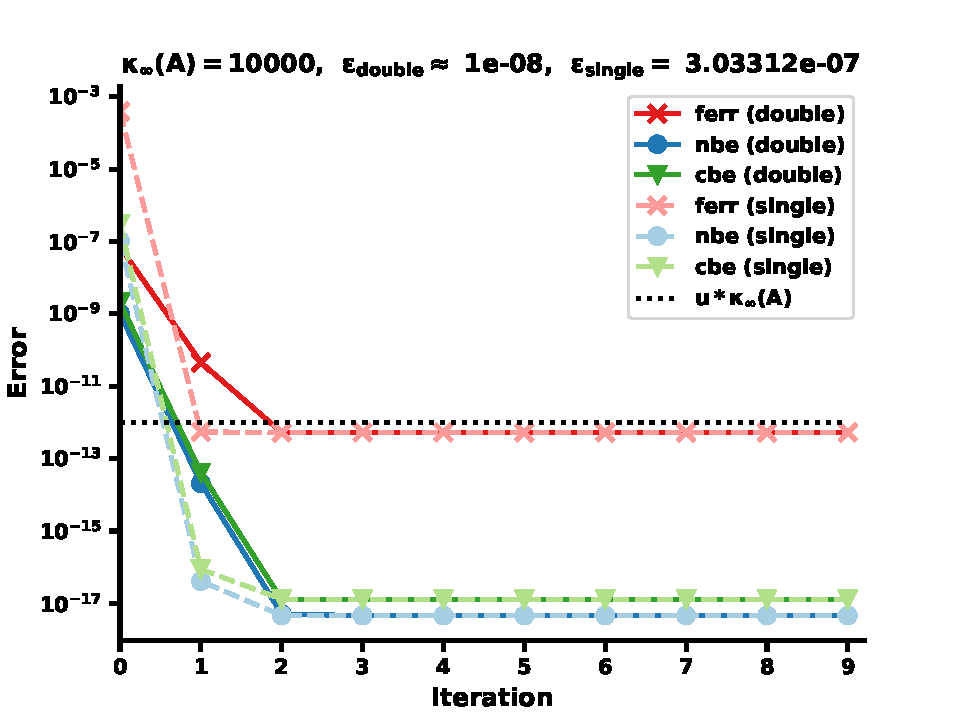
\includegraphics[width=\linewidth]{chapters/5_experiments/figures/GMRES512_e1_1s.pdf}
  \caption{$\epsilon_{double} \approx 10^{-8}$}
  \label{fig:lrirsg2_2}
\end{subfigure}
\caption[Mixed Precision Low-Rank GMRES-IR 2]{Comparison of hierarchical LU factorization in single and double precision. Measurements are obtained from a GMRES-based IR where $\kappa_\infty(A) \approx 10^4$.}
\label{fig:lrirsg2}
\end{figure}

\begin{figure}
\centering
\begin{subfigure}{.5\textwidth}
  \centering
  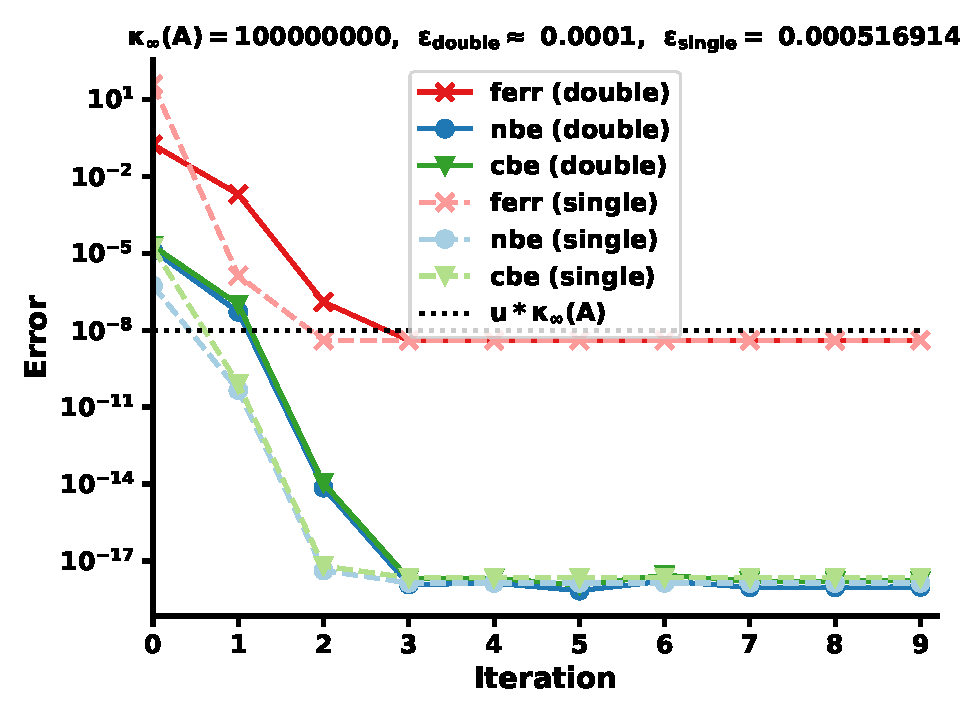
\includegraphics[width=\linewidth]{chapters/5_experiments/figures/GMRES512_e3_0s.pdf}
  \caption{$\epsilon_{double} \approx 10^{-2}$}
  \label{fig:lrirsg3_1}
\end{subfigure}%
\begin{subfigure}{.5\textwidth}
  \centering
  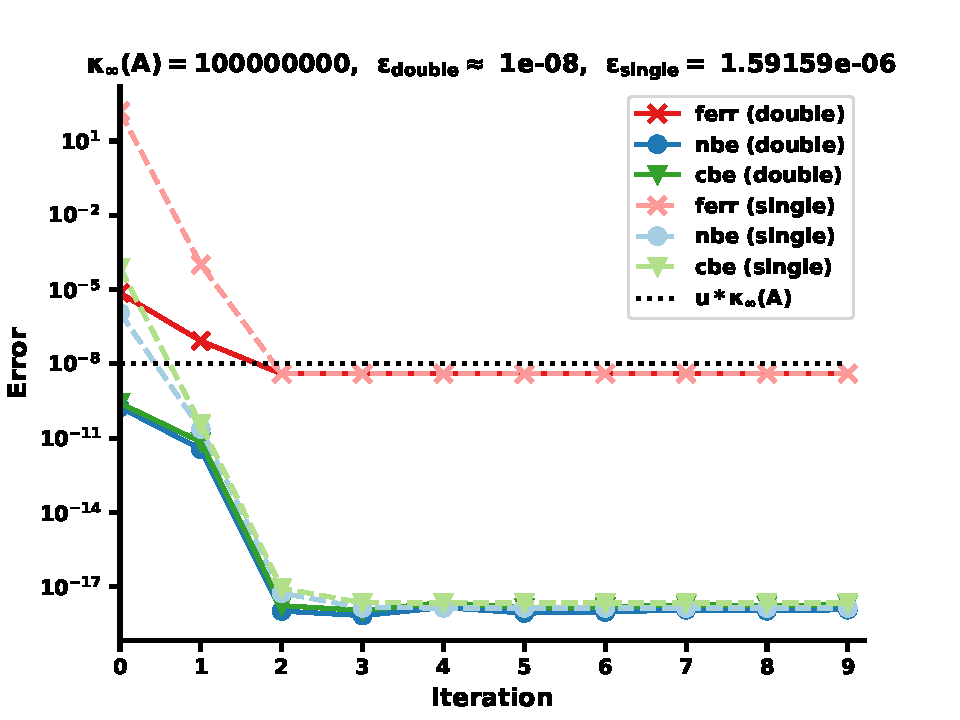
\includegraphics[width=\linewidth]{chapters/5_experiments/figures/GMRES512_e3_1s.pdf}
  \caption{$\epsilon_{double} \approx 10^{-8}$}
  \label{fig:lrirsg3_2}
\end{subfigure}
\caption[Mixed Precision Low-Rank GMRES-IR 3]{Comparison of hierarchical LU factorization in single and double precision. Measurements are obtained from a GMRES-based IR where $\kappa_\infty(A) \approx 10^8$.}
\label{fig:lrirsg3}
\end{figure}

Perhaps the most interesting observation to be made is that despite the lower precision used for the factorization, convergence can sometimes be achieved in less iterations (see Figures~\hyperref[fig:lrirsg2_2]{\ref{fig:lrirsg2_2}} \& \hyperref[fig:lrirsg3_1]{\ref{fig:lrirsg3_1}}). This suggests that the correction equation is solved at a higher accuracy in those cases, in spite of the initial error being larger. Since the GMRES part of the algorithm basically works independently from $u_f$ this is slightly surprising and the cost of the faster convergence might be associated with a higher number of inner GMRES iterations. Investigating this hypothesis, the results illustrated in Figure~\hyperref[fig:lr_irs_iter]{\ref{fig:lr_irs_iter}} were obtained.

\begin{figure}[h]
    \centering
    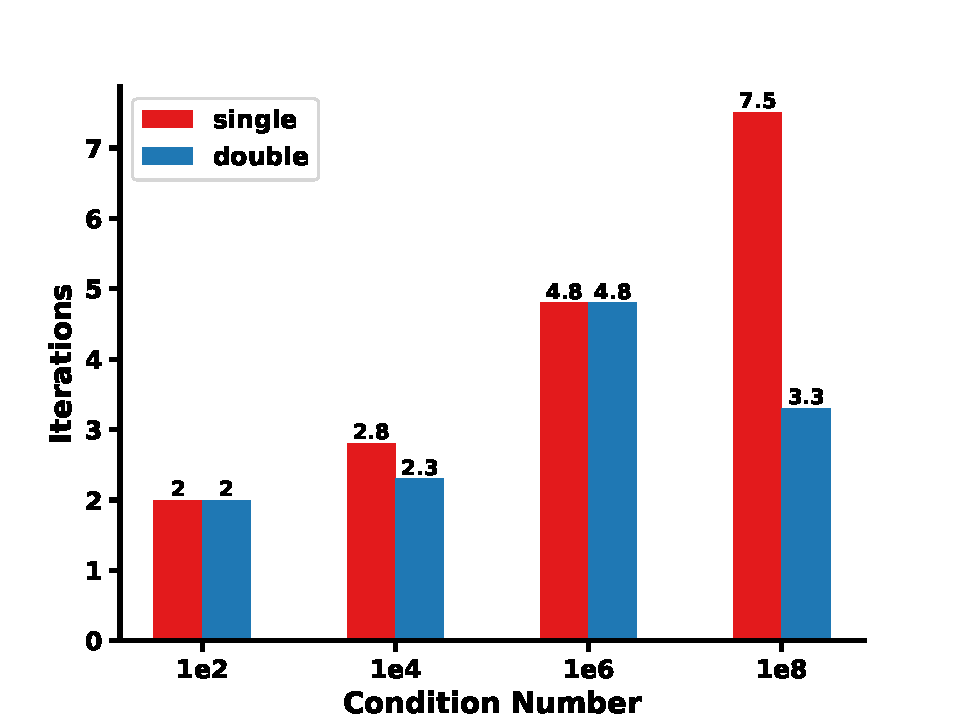
\includegraphics[width=0.7\linewidth]{chapters/5_experiments/figures/GMRES_iter.pdf}
    \caption[Mixed Precision Low-Rank IR - GMRES Iterations]{Comparison calculating the LU decomposition in single/double precision for $1024 \times 1024$ matrices with varying condition number. The iteration count is given as the average across all accuracy settings (i.e. $\epsilon$)}
    \label{fig:lr_irs_iter}
\end{figure}

Significant differences are only observable for a condition number $\kappa_\infty(A) \geq u_f^{-1}$, where GMRES needs considerable more iterations for the low precision LU factors. This is a natural consequence of the quality of the preconditioner that deteriorates in such a case in a way that it can not be used for LU-based iterative refinement anymore. In other words, while the double precision LU factors retain some information that reduces the condition number of $A$ considerable, the single precision ones only guarantee $ \kappa(\hat{U}^{-1}\hat{L}^{-1}A)\approx 1 + \kappa(A)u$. Hence, more GMRES iterations are necessary since $\kappa(\hat{U}^{-1}\hat{L}^{-1}A$ becomes increasingly ill-conditioned.

On the other hand, some slight variations in the number of GMRES steps can be observed, even for matrices with lower condition numbers (as for example in the $\kappa_\infty(A) \approx 10^4$ case). Those coincide with the previously attested lower IR iteration count, because the additional GMRES step presumably solves the correction equation at a higher accuracy then the prescribed minimum. Thus, a larger correction step can be taken, decreasing the number of overall iterations to achieve convergence (a similar effect becomes visible if the mentioned GMRES threshold is adjusted). In principle, this phenomenon is independent of the precision used, as it is a simple trade between an IR and a GMRES iteration (more GMRES iterations requiere less IR steps and vice versa). The effects are thus considered negligible, since the never amount to more than a single additional iteration.

The final part of this section aims to examine the importance of the high precision computations (i.e. $u_r$) used within the proposed algorithms. Iterative refinement is known to work in a fixed precision setting \cite{skeel_iterative_1980} as well and, due to the high cost associated with the higher precision calculations, the question arises whether those are truly necessary or not. For this purpose, a three precision low-rank approximation approach is used, downgrading the third precision to be equal to working precision (i.e. $u_f = single$, $u=u_r=double$). Only limited experiments have been conducted with these settings, but exemplary results can be seen in Figure~\hyperref[fig:lu_high]{\ref{fig:lu_high}} for LU-based and Figure~\hyperref[fig:gmres_high]{\ref{fig:gmres_high}} for GMRES-based iterative refinement.

\begin{figure}[h]
\centering
\begin{subfigure}{.5\textwidth}
  \centering
  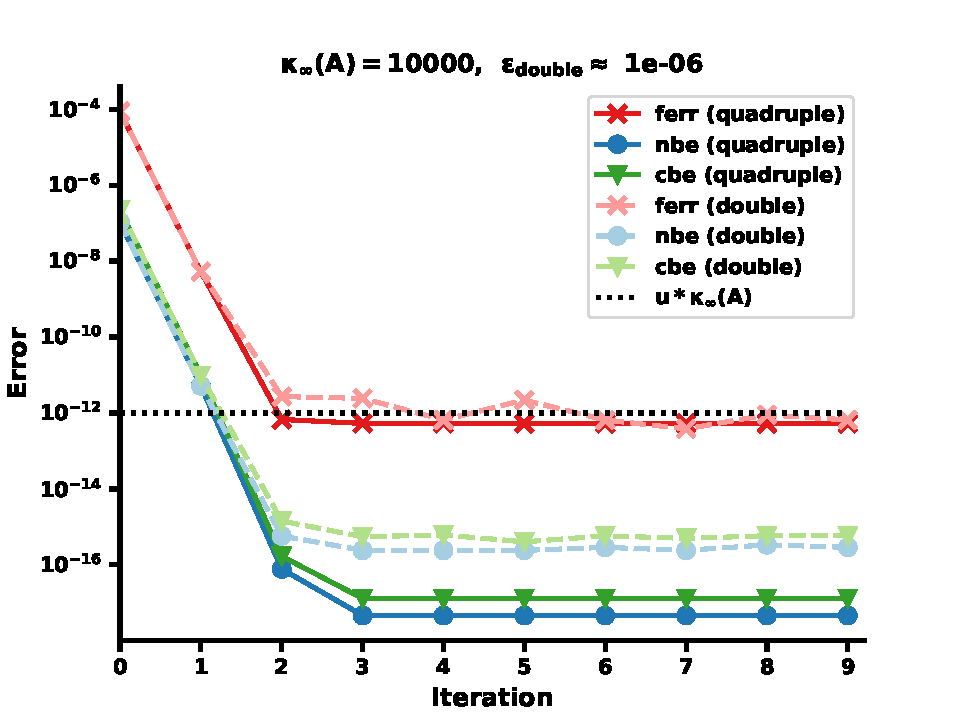
\includegraphics[width=\linewidth]{chapters/5_experiments/figures/LU_high.pdf}
  \caption{LU-based IR}
  \label{fig:lu_high}
\end{subfigure}%
\begin{subfigure}{.5\textwidth}
  \centering
  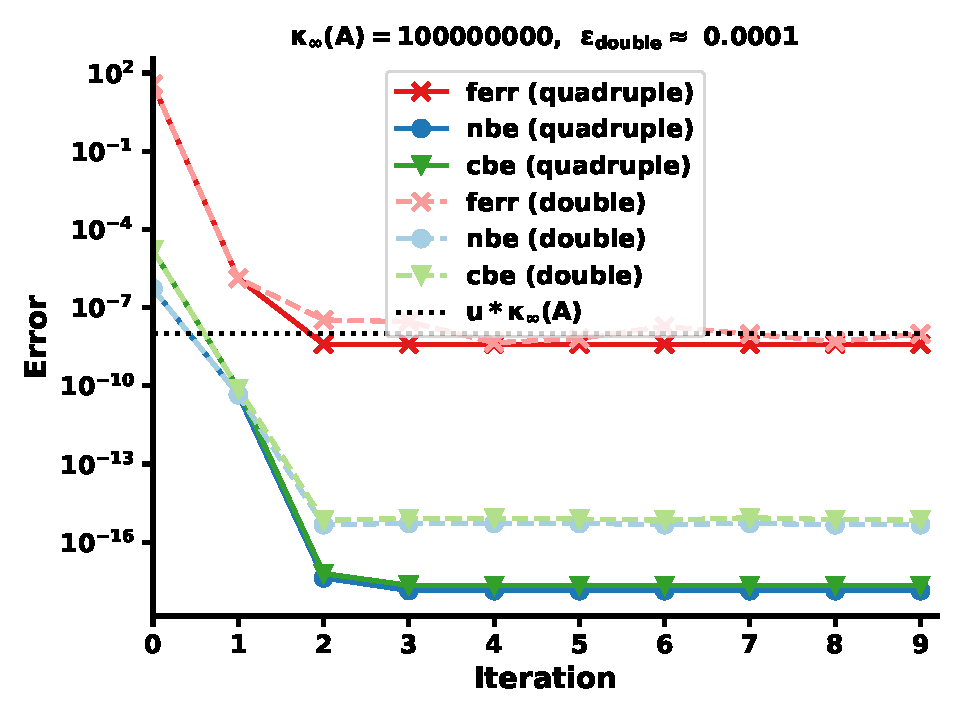
\includegraphics[width=\linewidth]{chapters/5_experiments/figures/GMRES_high.pdf}
  \caption{GMRES-based IR}
  \label{fig:gmres_high}
\end{subfigure}
\caption[Mixed Precision Low-RankIR (without high precision)]{Comparing different settings for $u_r$ within three precision LU-/GMRES-based iterative refinement for a $512 \times 512$ matrix with varying condition number and accuracy threshold.}
\label{fig:lr_high}
\end{figure}

Although the same error bound can be maintained for the forward error, the obtained backward errors, both norm- and component-wise are clearly worse than in the high precision case. However, even if they are not accurate to working precision, they still decrease considerably from their initial value and, depending on the requirements of the application, might be sufficient for some use-cases. Especially if speed is favoured over accuracy, those variants are preferable since they do not suffer from the slowdown incurred by the high precision arithmetics. From the conducted experiments, it seems like the implications of reduced residual accuracy affect LU- and GMRES-based IR refinement equally, not causing any further differences between those methods.

This is slightly surprising, since GMRES-based IR relies on those high precision calculations to a greater account, using them for applying the preconditioner in addition to matrix-vector products. Those findings suggest that the bound presented in \cite{carson_new_2017} are not necessarily sharp and high precision computations might be avoidable for certain problems. Indeed, for the set of matrices used in this research simply replacing the quadruple calculations within the GMRES part of the algorithm by the corresponding double precision ones, did not change any of the presented results (given that the residuals calculation still remained in quadruple precision). While this might not be applicable for the general case, the results obtained in this research indicate that for certain matrices the same error bound are applicable, even if GMRES-IR is only conducted in two precisions. However, further research would be necessary before any definite conclusion can be drawn. 